\documentclass[a4paper, 11pt]{report}
\usepackage[utf8]{inputenc}
\usepackage[T1]{fontenc}

\usepackage[margin=1in]{geometry}
\usepackage{amsmath, amsfonts, amsthm, amssymb, amsxtra}

\usepackage{graphicx}
\usepackage{float}

\usepackage[dvipsnames]{xcolor}

\usepackage{tabularray}
\usepackage{enumitem}
\usepackage{multicol}

\usepackage{notomath}
\usepackage{minted}

\usepackage{hyperref}
\hypersetup{hidelinks}

\usepackage{tikz}
\usepackage{pgfplots}
\pgfplotsset{compat=1.18}
\usetikzlibrary{intersections, angles, calc, positioning}
\usetikzlibrary{shapes.geometric, arrows.meta}
\usetikzlibrary{decorations.pathmorphing, decorations.pathreplacing}

\setlength{\parindent}{0pt}
\setlength{\parskip}{5pt}

\setcounter{chapter}{5}

\makeatletter
\newcommand{\type}[1]{\def\@type{#1}}

\renewcommand*{\maketitle}{%
\vspace{-0.5cm}
\begin{tikzpicture}[remember picture, overlay]
    \node[anchor=south, align=center] (date) at ($(current page.north) + (0,-110pt)$) {\@date};
    \node[anchor=south, align=center, font=\itshape] (author) at (date.north) {\@author};
    \node[above=10pt of author, align=center, font=\scshape] (type) {\@type};
    \node[anchor=south, align=center, font=\bfseries\large] (title) at (type.north) {\@title};
    \node[anchor=west] (logo) at ($(current page.north west) + (\Gm@lmargin, -67pt)$) {
\includegraphics[height=3cm]{ufs_vertical_positiva.eps}};
    \draw ($(current page.north west) + (\Gm@lmargin, -120pt)$) -- ($(current page.north east) + (-\Gm@lmargin, -120pt)$);
\end{tikzpicture}
\vspace{45pt}
}%
\makeatother

\title{Cálculo Numérico II}
\type{Lista 1}
\author{Bruno Sant'Anna}
\date{15 de fevereiro de 2024}

\begin{document}
\maketitle

\begin{center}
    \textcolor{teal}{\fbox{\Large QUESTÕES UTILIZANDO O PYTHON}}
\end{center}

\setcounter{section}{1}
\section{Método de Euler}
% Dado um problema de valor inicial da forma
% \[
%     \left\{
%         \begin{array}{ll}
%             y' = f(t,y) & t_0 \leqslant t \leqslant t_N\\
%             y(t_0) = \alpha &
%         \end{array}
%     \right.
% \]
% Podemos usar o método de Euler para aproximar a solução do \textsc{pvi} por pontos descontinuos da seguinte forma.
% \[
%     \begin{aligned}
%         w_0 &= \alpha\\
%         w_{i+1} &= w_i + hf(t_i, w_i)
%     \end{aligned}
% \]
% para todo $i = 0, 1,\dots, N-1$, onde $N$ representa o número de pontos na solução aproximada, $h = \frac{1}{2}(t_N - t_0)$ é o passo, e $t_{i} = t_0 + ih$.

\begin{enumerate}[leftmargin=*, label=\textbf{\arabic*.}]
    % \item Use o método de euler para aproximar as soluções de cada problema de valor inicial
    % \begin{enumerate}[label=  \alph*.]
    %     \item $y' = te^{3t} - 2y$, $\; 0 \leqslant t \leqslant 1$, $\; y(0) = 0$ com $h=0.5$
        
    %     \begin{align*}
    %         w_0 &= 0 \\
    %         w_1 &= 0 + 0.5e^{3 \cdot 0.5} - 2 \cdot 0 = 1.1204 \\
    %         w_2 &= 1.1204 + 1e^{3 \cdot 1} - 2 \cdot 1.1204 = 10.0427
    %     \end{align*}

    %     \item[d.]  $y' = \cos 2t - \sin 3t$, $\; 0 \leqslant t \leqslant 1$, $\; y(0) = 1$ com $h=0.25$

    %     \begin{align*}
    %         w_0 &= 1 \\
    %         w_1 &= \cos (2 \cdot 0.25) - \sin (3 \cdot 0.25) = 1.3898 \\
    %         w_2 &= \cos (2 \cdot 0.5) - \sin (3 \cdot 0.5) = 1.7742 \\
    %         w_3 &= \cos (2 \cdot 0.75) - \sin (3 \cdot 0.75) = 1.9864 \\
    %         w_4 &= \cos (2 \cdot 1) - \sin (3 \cdot 1) = 1.9144
    %     \end{align*}
    % \end{enumerate}

    \item[9.] Dado o problema de valor incial
    \[
        \left\{
        \begin{array}{ll}
            y' = \frac{2y}{t} + t^2 e^t & t \in [1,2]\\
            y(1) = 0 &
        \end{array}
        \right.
    \]
    com solução exata $y(t) = t^2 (e^t - e)$
    \begin{enumerate}[leftmargin=*, label=\alph*.]
        \item Use o método de euler com $h = 0.1$ para uma aproximação da solução e compare com os valores reais de $y$
        
        \begin{minipage}{0.42\columnwidth}
            \begin{tblr}{
                colspec={crrc},
                hline{1,Z} = {1pt, solid},
                hline{2} = {0.5pt, solid},
                row{1} = {c, abovesep=3pt, belowsep=3pt}
                }   
                $t_i$ & $w_i$   & $y(t_i)$ & $|y(t_i) - w_i|$\\
                1.0   & 0.0000  & 0.0000   & 0.0000 \\
                1.1   & 0.2718  & 0.3459   & 0.0740 \\
                1.2   & 0.6847  & 0.8666   & 0.1818 \\
                1.3   & 1.2769  & 1.6072   & 0.3302 \\
                1.4   & 2.0935  & 2.6203   & 0.5268 \\
                1.5   & 3.1874  & 3.9676   & 0.7802 \\
                1.6   & 4.6208  & 5.7209   & 1.1001 \\
                1.7   & 6.4663  & 7.9638   & 1.4974 \\
                1.8   & 8.8091  & 10.7936  & 1.9845 \\
                1.9   & 11.7479 & 14.3230  & 2.5750 \\
                2.0   & 15.3982 & 18.6830  & 3.2848
            \end{tblr}
        \end{minipage}
        \hfill
        \begin{minipage}{0.53\columnwidth}
            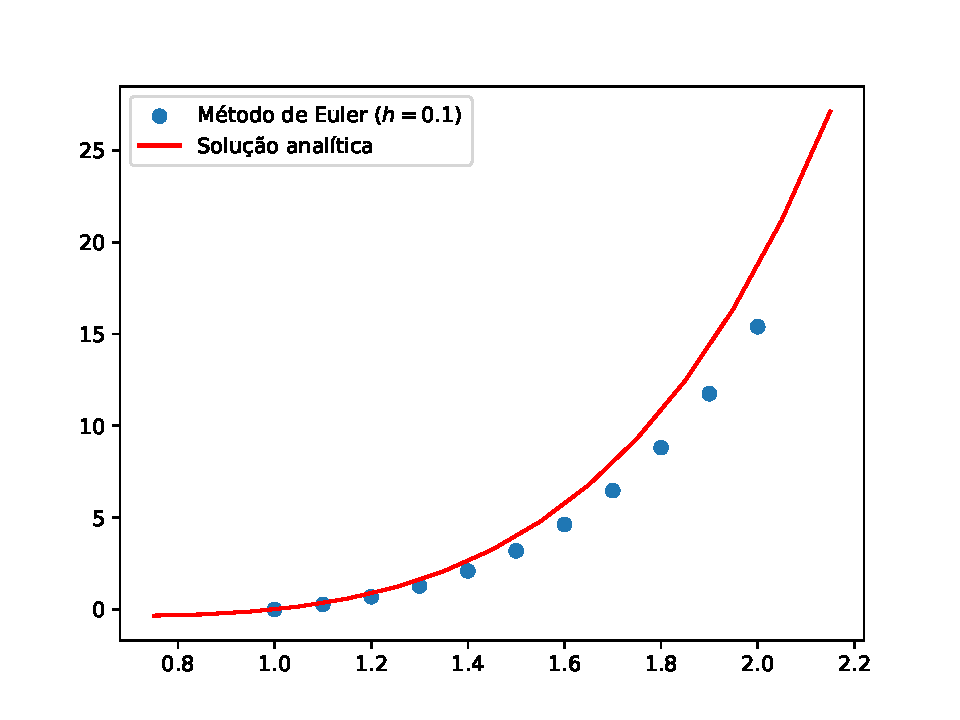
\includegraphics[width=\columnwidth]{../metodo de euler/q9.pdf}
        \end{minipage}
        
        \item Utilize as respostas geradas na parte (a) e a interpolação linear para encontrar a aproximação dos seguintes valores de $y$ e compare-os com os valores reais.
        \begin{multicols}{3}
            \begin{enumerate}[leftmargin=12pt, label=\roman*.]
                \item $y(1.04)$
                \item $y(1.55)$
                \item $y(1.97)$
            \end{enumerate}
        \end{multicols}

        Utilizando o método de Neville para interpolação linear temos que
        \begin{center}
            \begin{tblr}{
                colspec={crrc},
                hline{1,Z} = {1pt, solid},
                hline{2} = {0.5pt, solid},
                row{1} = {c, abovesep=3pt, belowsep=3pt}
                }   
                $t_i$  & $w_i$    & $y(t_i)$  & $|y(t_i) - w_i|$\\
                1.04   &  0.1087  &  0.1199   & 0.0112 \\
                1.55   &  3.9041  &  4.7886   & 0.8839 \\
                1.97   & 13.8052  & 17.2792   & 3.4740 \\
            \end{tblr}
        \end{center}

        \item Calcule o valor de $h$ necessário para que $|y(t_i) - w_i| \leqslant 0.1$
    \end{enumerate}

    \item[16.] Em um circuito com tensão aplicada $\mathcal E$ e com resistência $R$, indutância $L$ e capacitância $C$, a corrente $i$ satisfaz a equação diferencial
    \[
        \frac{di}{dt} = C\frac{d^2 \mathcal E}{dt^2} + \frac{1}{R}\frac{d\mathcal{E}}{dt} + \frac{1}{L}\mathcal E
    \]
    Suponha que $C = 0.3 \mathrm{F}$, $R = 1.4 \Omega$, $L = 1.7 \mathrm{H}$ e que a tensão seja dada por
    \[
        \mathcal{E}(t) = e^{-0.06\pi t}\sin(2t - \pi)
    \]
    se $i(0) = 0$ encontre a corrente $i$ para os valores $0.1 k$ onde $k = 0,1,\dots,100$

    \[
        \frac{\mathrm{d} \mathcal{E}}{\mathrm{d}t} = -e^{-0.06\pi t}(0.06\pi \sin(2t- \pi) + 2\cos(2t- \pi))
    \]
    \[
        \frac{\mathrm{d}^2 \mathcal{E}}{\mathrm{d}t^2} = -e^{-0.06\pi t}(0.06\pi \sin(2t - \pi) - 4\sin(2t - \pi) + 2\cos(2t - \pi) + 0.12\pi \cos(2t - \pi))
    \]
    \begin{center}
        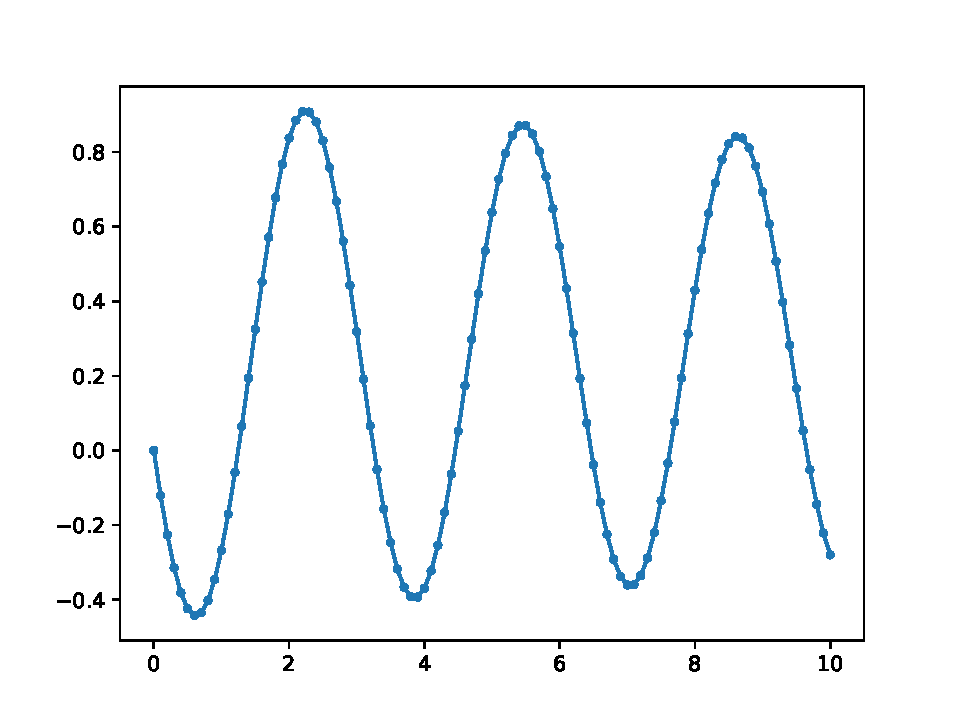
\includegraphics[width=0.75\columnwidth]{../metodo de euler/q16.pdf}
    \end{center}
\end{enumerate}

\section{Método de Taylor}
% Dado um problema de valor inicial da forma
% \[
%     \left\{
%         \begin{array}{ll}
%             y' = f(t,y) & t_0 \leqslant t \leqslant t_N\\
%             y(t_0) = \alpha &
%         \end{array}
%     \right.
% \]
% Podemos usar o método de Taylor para aproximar a solução do \textsc{pvi} por pontos descontinuos da seguinte forma.
% \[
%     \begin{aligned}
%         w_0 &= \alpha\\
%         w_{i+1} &= w_i + hf(t_i, w_i) + \tfrac{\, h^2}{2}f'(t_i, w_i)
%     \end{aligned}
% \]
% para todo $i = 0, 1,\dots, N-1$.

\begin{enumerate}[leftmargin=*]
    \item[9.] Dado o problema de valor incial
    \[
        \left\{
        \begin{array}{ll}
            y' = \frac{2y}{t} + t^2 e^t & t \in [1,2]\\
            y(1) = 0 &
        \end{array}
        \right.
    \]
    com solução exata $y(t) = t^2 (e^t - e)$
    \begin{enumerate}[leftmargin=*, label=\alph*.]
        \item Use o método de Taylor de segunda ordem com $h = 0.1$ para encontrar uma aproximação da solução e compare-a com os valores reais de $y$.

        \begin{minipage}{0.42\columnwidth}
            \begin{tblr}{
                colspec={crrc},
                hline{1,Z} = {1pt, solid},
                hline{2} = {0.5pt, solid},
                row{1} = {c, abovesep=3pt, belowsep=3pt}
                }   
                $t_i$ & $w_i$   & $y(t_i)$ & $|y(t_i) - w_i|$\\
                1.0   & 0.0000  & 0.0000   & 0.0000 \\
                1.1   & 0.3397  & 0.3459   & 0.0061 \\
                1.2   & 0.8521  & 0.8666   & 0.0144 \\
                1.3   & 1.5817  & 1.6072   & 0.0254 \\
                1.4   & 2.5809  & 2.6203   & 0.0393 \\
                1.5   & 3.9109  & 3.9676   & 0.0566 \\
                1.6   & 5.6430  & 5.7209   & 0.0778 \\
                1.7   & 7.8603  & 7.9638   & 0.1034 \\
                1.8   & 10.6595 & 10.7936  & 0.1341 \\
                1.9   & 14.1526 & 14.3230  & 0.1703 \\
                2.0   & 18.4699 & 18.6830  & 0.2131
            \end{tblr}
        \end{minipage}
        \hfill
        \begin{minipage}{0.53\columnwidth}
            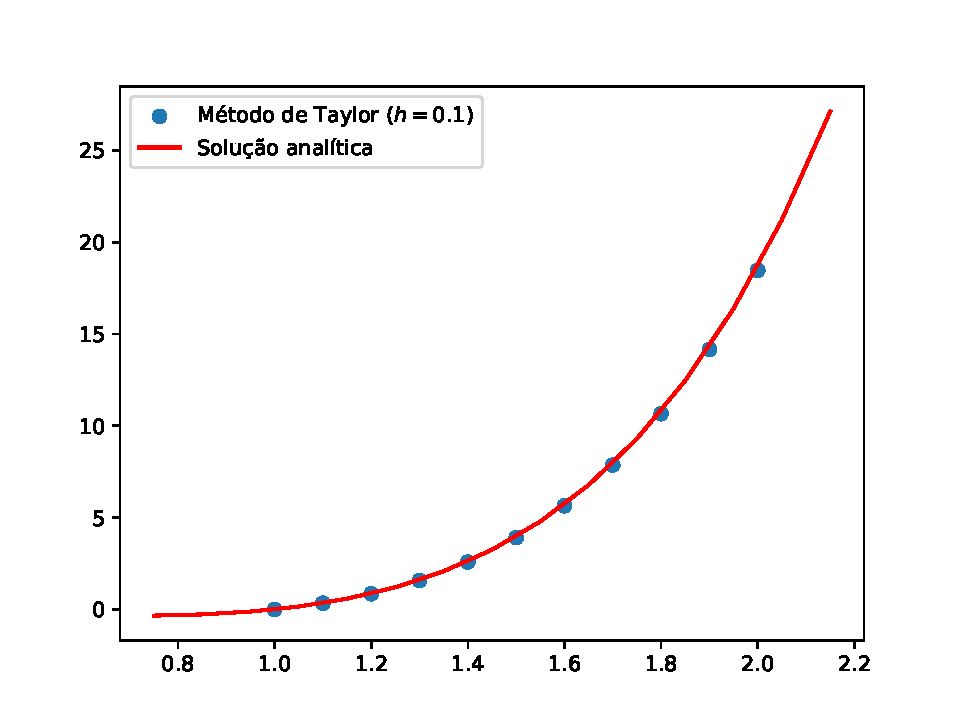
\includegraphics[width=\columnwidth]{../metodo de taylor/q9a.pdf}
        \end{minipage}

        \item Use as respostas geradas na parte (a) e a interpolação linear para encontrar aproximações de $y$ nos valores a seguir e compare-as com os valores reais de $y$.
        \begin{multicols}{3}
            \begin{enumerate}[leftmargin=12pt, label=\roman*.]
                \item $y(1.04)$
                \item $y(1.55)$
                \item $y(1.97)$
            \end{enumerate}
        \end{multicols}

        Utilizando o método de Neville para interpolação linear, temos que
        \begin{center}
            \begin{tblr}{
                colspec={crrc},
                hline{1,Z} = {1pt, solid},
                hline{2} = {0.5pt, solid},
                row{1} = {c, abovesep=3pt, belowsep=3pt}
                }   
                $t_i$  & $w_i$    & $y(t_i)$  & $|y(t_i) - w_i|$\\
                1.04   &  0.1359  &  0.1199   & 0.016 \\
                1.55   &  4.7770  &  4.7886   & 0.011 \\
                1.97   & 17.1748  & 17.2792   & 0.104 \\
            \end{tblr}
        \end{center}

        \item Use o método de Taylor de quarta ordem com $h = 0.1$ para encontrar uma aproximação da solução e compare-a com os valores reais de $y$.

        \begin{minipage}{0.42\columnwidth}
            \begin{tblr}{
                colspec={crrc},
                hline{1,Z} = {1pt, solid},
                hline{2} = {0.5pt, solid},
                row{1} = {c, abovesep=3pt, belowsep=3pt}
                }   
                $t_i$ & $w_i$   & $y(t_i)$ & $|y(t_i) - w_i|$\\
                1.0 & 0.0000  & 0.0000  & 0.0000 \\
                1.1 & 0.3462  & 0.3459  & 0.0003 \\
                1.2 & 0.8672  & 0.8666  & 0.0006 \\
                1.3 & 1.6082  & 1.6072  & 0.0010 \\
                1.4 & 2.6219  & 2.6204  & 0.0015 \\
                1.5 & 3.9697  & 3.9677  & 0.0021 \\
                1.6 & 5.7237  & 5.7210  & 0.0027 \\
                1.7 & 7.9673  & 7.9639  & 0.0034 \\
                1.8 & 10.7979 & 10.7936 & 0.0043 \\
                1.9 & 14.3282 & 14.3231 & 0.0052 \\
                2.0 & 18.6893 & 18.6831 & 0.0062 
            \end{tblr}
        \end{minipage}
        \hfill
        \begin{minipage}{0.53\columnwidth}
            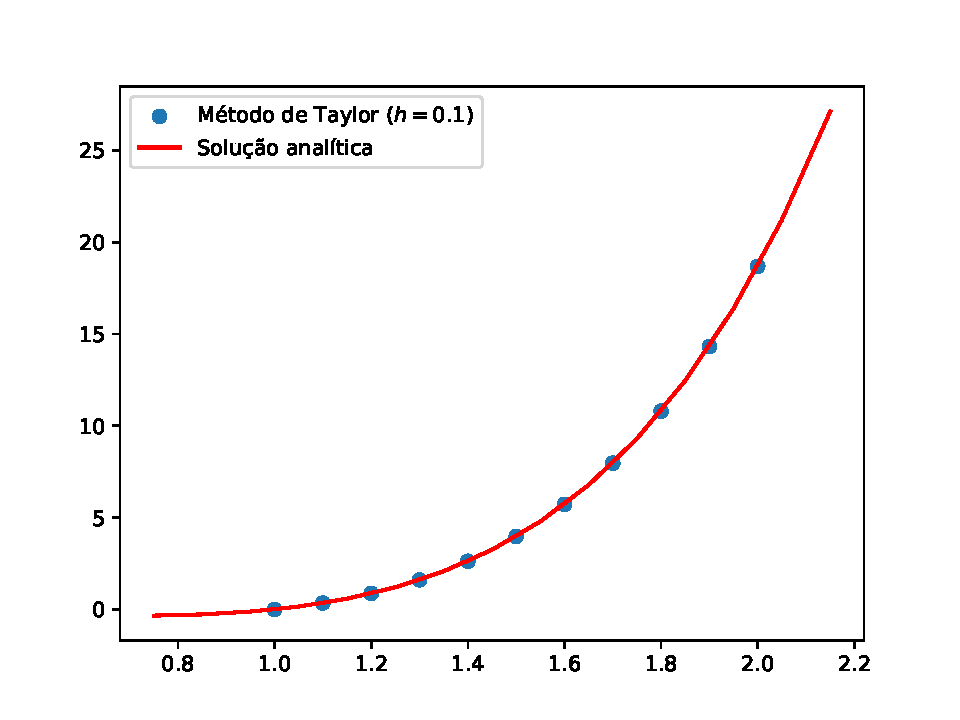
\includegraphics[width=\columnwidth]{../metodo de taylor/q9c.pdf}
        \end{minipage}

        % \item Use as respostas geradas na parte (c) e a interpolação cúbica de Hermite para encontrar aproximações de $y$ nos valores a seguir e compare-as com os valores reais de $y$.
        % \begin{multicols}{3}
        %     \begin{enumerate}[leftmargin=12pt, label=\roman*.]
        %         \item $y(1.04)$
        %         \item $y(1.55)$
        %         \item $y(1.97)$
        %     \end{enumerate}
        % \end{multicols}
    \end{enumerate}

    \item[11.] Use o método de Taylor com $h = 0.1$ para encontrar uma aproximação da solução de
    \[y' = 1 + t \sin (ty), \;\; 0 \leqslant t \leqslant 2, \;\; y(0) = 0\]

    Para utlizar o método de Taylor de segunda ordem precisamos calcular $y''$, partindo de $y' = 1 + t \sin (ty)$ temos
    \begin{align*}
        y'' &= \sin (ty) + t \cos (ty) y'\\
            &= \sin (ty) + (1 + t \sin (ty)) t \cos (ty)
    \end{align*}

    \begin{minipage}{0.36\columnwidth}
        \begin{tblr}{
            colspec={crrc},
            hline{1,Z} = {1pt, solid},
            hline{2} = {0.5pt, solid},
            vline{3} = {0.5pt, solid},
            row{1} = {c, abovesep=3pt, belowsep=3pt},
            }   
            $t_i$ & $w_i$   & $t_i$    & $w_i$\\
            0.0 & 0.0000    &          &        \\
            0.1 & 0.1000    & 1.1      & 1.4539 \\
            0.2 & 0.2002    & 1.2      & 1.6683 \\
            0.3 & 0.3016    & 1.3      & 1.8714 \\
            0.4 & 0.4057    & 1.4      & 2.0382 \\
            0.5 & 0.5146    & 1.5      & 2.1525 \\
            0.6 & 0.6312    & 1.6      & 2.2132 \\
            0.7 & 0.7590    & 1.7      & 2.2283 \\
            0.8 & 0.9022    & 1.8      & 2.2080 \\
            0.9 & 1.0647    & 1.9      & 2.1614 \\
            1.0 & 1.2493    & 2.0      & 2.0951
        \end{tblr}
    \end{minipage}
    \hfill
    \begin{minipage}{0.62\columnwidth}
        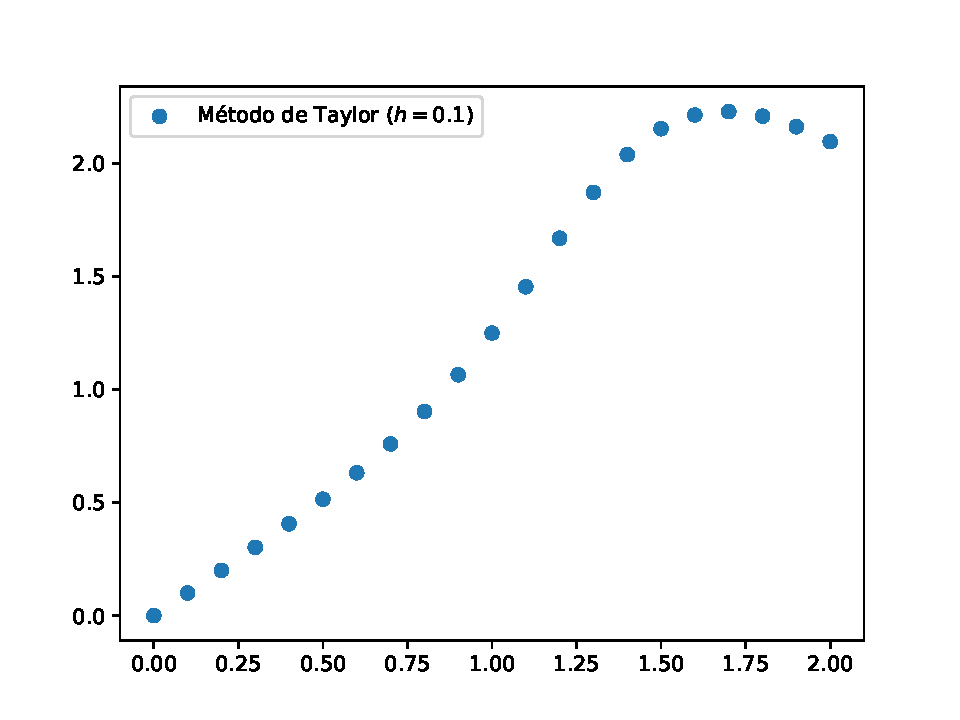
\includegraphics[width=\columnwidth]{../metodo de taylor/q11.pdf}
    \end{minipage}


    \item[12.] Um projétil de massa $m = 0.11 \mathrm{kg}$ jogado verticalmente para cima com velocidade inicial $v(0) = 8 \mathrm{m/s}$ tem sua velocidade diminuida pela força da gravidade, $F_g = -mg$, e pela resistência do ar, $F_r = -kv|v|$, em que $g = 9.8 \mathrm{m/s}^2$ e $k = 0.002 \mathrm{kg/m}$.
    A equação diferencial para velocidade $v$ é dada por
    \begin{equation} \label{eq:projetil}
        mv' = -mg - kv|v|.
    \end{equation}
    \begin{enumerate}[leftmargin=*, label=\alph*.]
        \item Encontre a velocidade após 0.1, 0.2,\dots,1.0 s.
        \begin{center}
            \begin{tblr}{
                colspec={crrc},
                hline{1,Z} = {1pt, solid},
                hline{2} = {0.5pt, solid},
                vline{3} = {0.5pt, solid},
                row{1} = {c, abovesep=3pt, belowsep=3pt}
                }   
                $t_i$ & $w_i$   & $t_i$ & $w_i$   \\
                0.1   &  6.8876 & 0.6   &  1.7154 \\ 
                0.2   &  5.8080 & 0.7   &  0.7270 \\ 
                0.3   &  4.7557 & 0.8   & -0.2552 \\ 
                0.4   &  3.7257 & 0.9   & -1.2355 \\
                0.5   &  2.7137 & 1.0   & -2.2149 \\
            \end{tblr}
        \end{center}

        \item Com precisão de um décimo de segundo determine quando o projétil alcança sua altura máxima e começa a cair
        
        \begin{minipage}{0.42\columnwidth}
            A altura máxima é atingida quando $v = 0$, pelos pontos calculados com o método de Taylor de segunda ordem, é possível ver que a altura máxima acontece entre 0.7 e 0.8s. Usando a reta de ajuste $-10.1160t + 7.8673$, temos que a altura máxima é atingida em 0.77s 
        \end{minipage}
        \hfill
        \begin{minipage}{0.53\columnwidth}
            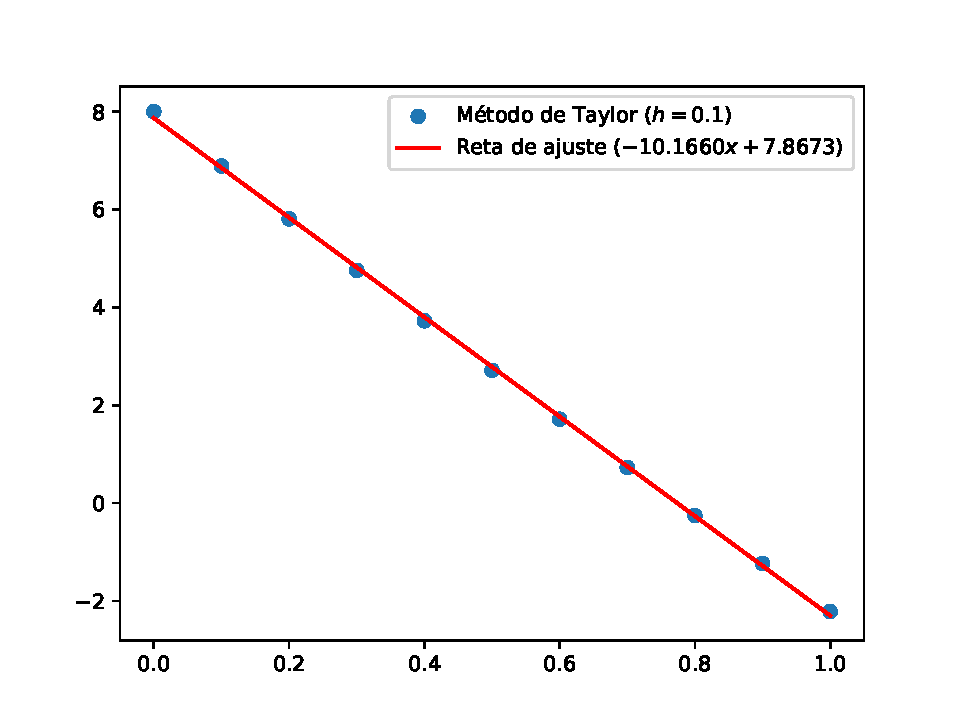
\includegraphics[width=\columnwidth]{../metodo de taylor/q12.pdf}
        \end{minipage}
    \end{enumerate}
\end{enumerate}

\section{Método de Runge-Kutta}
% Dado um problema de valor inicial da forma
% \[
%     \left\{
%         \begin{array}{ll}
%             y' = f(t,y) & t_0 \leqslant t \leqslant t_N\\
%             y(t_0) = \alpha &
%         \end{array}
%     \right.
% \]
% Podemos usar o método de Runge para aproximar a solução do \textsc{pvi} por pontos descontinuos da seguinte forma.
% \[
%     \begin{aligned}
%         w_0 &= \alpha\\
%         w_{i+1} &= w_i + \frac{1}{6}(k_1 + 2k_2 + 2k_3 + k_4)
%     \end{aligned}
% \]
% para todo $i = 0, 1,\dots, N-1$, onde
% \[
%     \begin{aligned}
%         k_1 &= hf(t_i, w_i)\\
%         k_2 &= hf(t_i + 0.5h, w_i + 0.5k_1)\\
%         k_3 &= hf(t_i + 0.5h, w_i + 0.5k_2)\\
%         k_4 &= hf(t_{i+1} + 0.5h, w_i + k_3)
%     \end{aligned}
% \]
% Uma outra forma é o método de Euler modificado, dado por
% \[
%     \dots
% \]
% Ou o método do ponto médio
% \[
%     \dots
% \]

\begin{enumerate}[leftmargin=*]
    \item[3.] Use o método de Euler modificado pr encontrar aproximações das soluções de cada um dos seguintes problemas de valor inicial e compare os resultados com os valores reais
    \begin{enumerate}[leftmargin=*]
        \item[a.] $y' = \frac{y}{t} - \left( \frac{y}{t} \right)^2$, $\; 1 \leqslant t \leqslant 2$, $\; y(1) = 1$ com $h=0.1$; solução real $y(t) = \frac{t}{1 + \ln t}$

        \begin{minipage}{0.42\columnwidth}
            \begin{tblr}{
                colspec={crrc},
                hline{1,Z} = {1pt, solid},
                hline{2} = {0.5pt, solid},
                row{1} = {c, abovesep=3pt, belowsep=3pt}
                }   
                $t_i$ & $w_i$   & $y(t_i)$ & $|y(t_i) - w_i|$\\
                1.0   & 1.0000  & 1.0000  & 0.0000 \\
                1.1   & 1.0041  & 1.0043  & 0.0001 \\
                1.2   & 1.0147  & 1.0150  & 0.0002 \\
                1.3   & 1.0295  & 1.0298  & 0.0003 \\
                1.4   & 1.0472  & 1.0475  & 0.0003 \\
                1.5   & 1.0669  & 1.0673  & 0.0004 \\
                1.6   & 1.0881  & 1.0884  & 0.0004 \\
                1.7   & 1.1103  & 1.1107  & 0.0004 \\
                1.8   & 1.1333  & 1.1337  & 0.0004 \\
                1.9   & 1.1568  & 1.1572  & 0.0004 \\
                2.0   & 1.1808  & 1.1812  & 0.0004
            \end{tblr}
        \end{minipage}
        \hfill
        \begin{minipage}{0.53\columnwidth}
            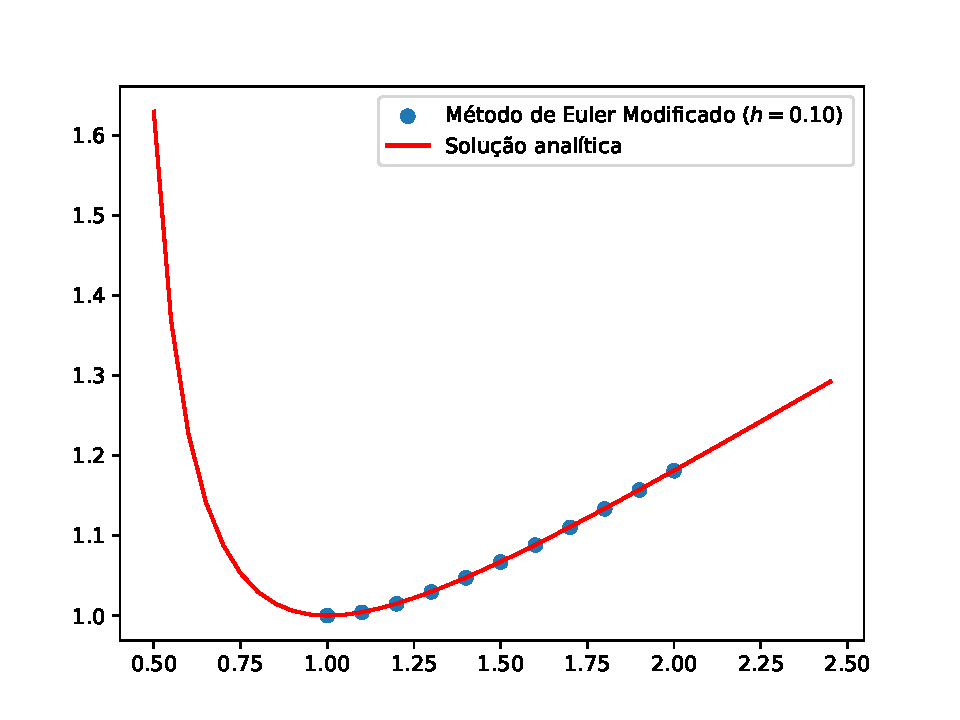
\includegraphics[width=\columnwidth]{../metodo de runge kutta/q3a.pdf}
        \end{minipage}
        \vspace{5pt}

        \item[b.] $y' = 1 + \frac{y}{t} + \left( \frac{y}{t} \right)^2$, $\; 1 \leqslant t \leqslant 2$, $\; y(1) = 0$ com $h=0.2$; solução real $y(t) = t \tan (\ln t)$

        \begin{minipage}{0.42\columnwidth}
            \begin{tblr}{
                colspec={crrc},
                hline{1,Z} = {1pt, solid},
                hline{2} = {0.5pt, solid},
                row{1} = {c, abovesep=3pt, belowsep=3pt}
                }   
                $t_i$ & $w_i$   & $y(t_i)$ & $|y(t_i) - w_i|$\\
                1.0   & 0.0000  & 0.0000   & 0.0000 \\
                1.2   & 0.2194  & 0.2212   & 0.0018 \\
                1.4   & 0.4850  & 0.4897   & 0.0046 \\
                1.6   & 0.8040  & 0.8128   & 0.0087 \\
                1.8   & 1.1849  & 1.1994   & 0.0146 \\
                2.0   & 1.6384  & 1.6613   & 0.0229 \\
                2.2   & 2.1789  & 2.2135   & 0.0346 \\
                2.4   & 2.8251  & 2.8766   & 0.0515 \\
                2.6   & 3.6025  & 3.6785   & 0.0760 \\
                2.8   & 4.5466  & 4.6587   & 0.1121 \\
                3.0   & 5.7076  & 5.8741   & 0.1665
            \end{tblr}
        \end{minipage}
        \hfill
        \begin{minipage}{0.53\columnwidth}
            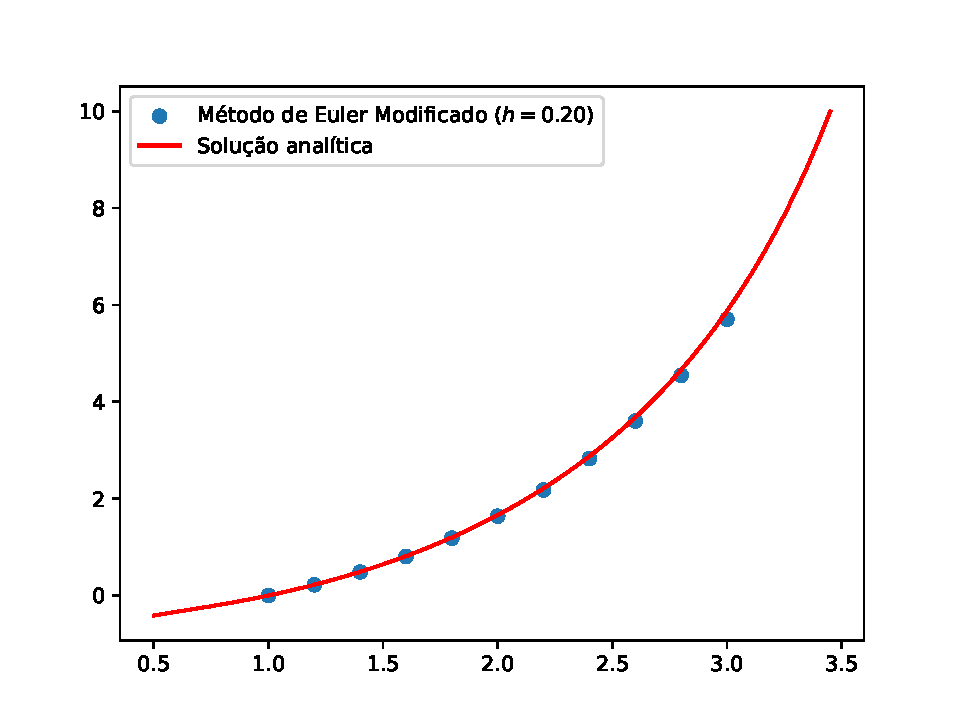
\includegraphics[width=\columnwidth]{../metodo de runge kutta/q3b.pdf}
        \end{minipage}
    \end{enumerate}
    \item[7.] Repita o exercício 3 usando o método do ponto médio
    \begin{enumerate}[leftmargin=*]
        \item[a.] $y' = \frac{y}{t} - \left( \frac{y}{t} \right)^2$, $\; 1 \leqslant t \leqslant 2$, $\; y(1) = 1$ com $h=0.1$; solução real $y(t) = \frac{t}{1 + \ln t}$

        \begin{minipage}{0.42\columnwidth}
            \begin{tblr}{
                colspec={crrc},
                hline{1,Z} = {1pt, solid},
                hline{2} = {0.5pt, solid},
                row{1} = {c, abovesep=3pt, belowsep=3pt}
                }   
                $t_i$ & $w_i$   & $y(t_i)$ & $|y(t_i) - w_i|$\\
                1.0   & 1.0000  & 1.0000   & 0.0000 \\
                1.1   & 1.0045  & 1.0043   & 0.0003 \\
                1.2   & 1.0153  & 1.0150   & 0.0004 \\
                1.3   & 1.0302  & 1.0298   & 0.0004 \\
                1.4   & 1.0480  & 1.0475   & 0.0005 \\
                1.5   & 1.0677  & 1.0673   & 0.0005 \\
                1.6   & 1.0889  & 1.0884   & 0.0005 \\
                1.7   & 1.1111  & 1.1107   & 0.0005 \\
                1.8   & 1.1341  & 1.1337   & 0.0005 \\
                1.9   & 1.1577  & 1.1572   & 0.0005 \\
                2.0   & 1.1817  & 1.1812   & 0.0005
            \end{tblr}
        \end{minipage}
        \hfill
        \begin{minipage}{0.53\columnwidth}
            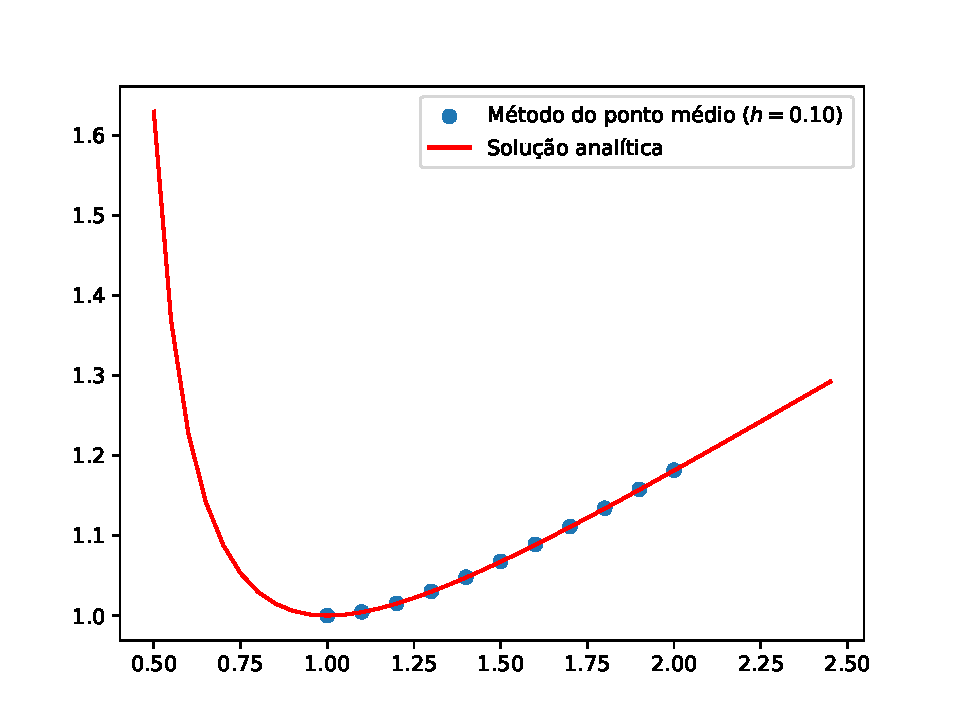
\includegraphics[width=\columnwidth]{../metodo de runge kutta/q7a.pdf}
        \end{minipage}
        \vspace{5pt}

        \item[b.] $y' = 1 + \frac{y}{t} + \left( \frac{y}{t} \right)^2$, $\; 1 \leqslant t \leqslant 2$, $\; y(1) = 0$ com $h=0.2$; solução real $y(t) = t \tan (\ln t)$

        \begin{minipage}{0.42\columnwidth}
            \begin{tblr}{
                colspec={crrc},
                hline{1,Z} = {1pt, solid},
                hline{2} = {0.5pt, solid},
                row{1} = {c, abovesep=3pt, belowsep=3pt}
                }   
                $t_i$ & $w_i$   & $y(t_i)$ & $|y(t_i) - w_i|$\\
                1.0   & 0.0000  & 0.0000   & 0.0000 \\
                1.2   & 0.2198  & 0.2212   & 0.0014 \\
                1.4   & 0.4862  & 0.4897   & 0.0035 \\
                1.6   & 0.8062  & 0.8128   & 0.0066 \\
                1.8   & 1.1884  & 1.1994   & 0.0110 \\
                2.0   & 1.6439  & 1.6613   & 0.0174 \\
                2.2   & 2.1869  & 2.2135   & 0.0266 \\
                2.4   & 2.8364  & 2.8766   & 0.0401 \\
                2.6   & 3.6185  & 3.6785   & 0.0600 \\
                2.8   & 4.5689  & 4.6587   & 0.0898 \\
                3.0   & 5.7386  & 5.8741   & 0.1355
            \end{tblr}
        \end{minipage}
        \hfill
        \begin{minipage}{0.53\columnwidth}
            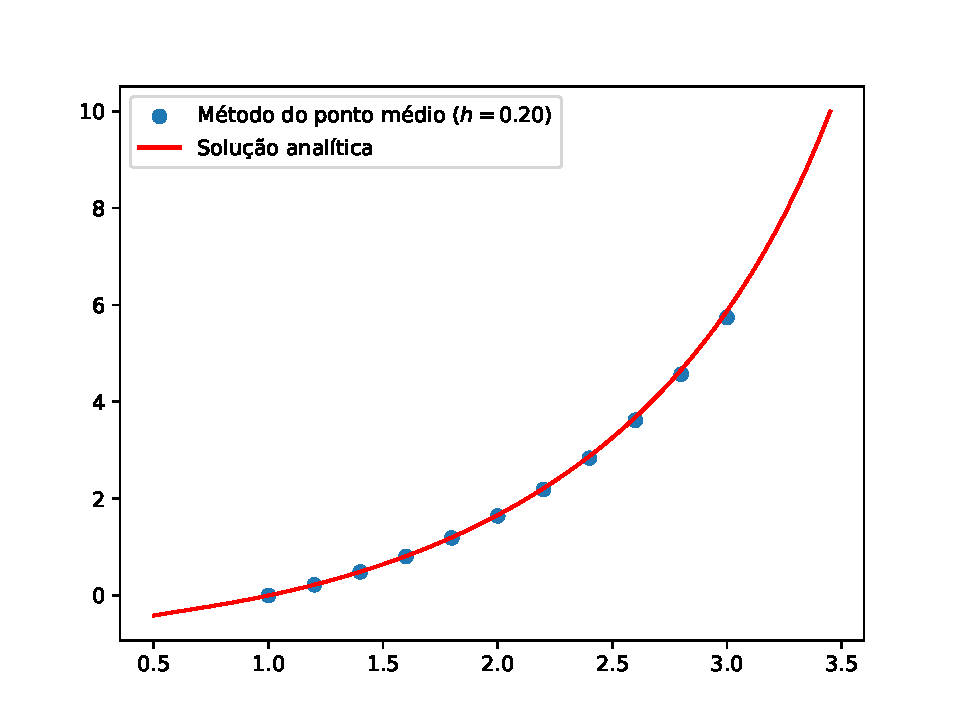
\includegraphics[width=\columnwidth]{../metodo de runge kutta/q7b.pdf}
        \end{minipage}
    \end{enumerate}

    \item[28.] A água escoa de um tanque cônico invertido com orifício circular a uma taxa de
    \[
        \frac{\mathrm{d} x}{\mathrm{d} t} = -0.6 \pi r^2 \sqrt{2g} \frac{\sqrt{x}}{A(x)}
    \]
    em que $r$ é o raio do orifício $x$ é altura do nível de líquido a partir do vértice do cone e $A(x)$ é a área da seção transversal do tanque $x$ unidades acima do orifício. Suponha que $r = 0.1 \,\mathrm{ft}$, $g = 32.1 \,\mathrm{ft/s^2}$ e que o tanque tenha um nível inicial de água de $8 \,\mathrm{ft}$ e volume inicial de $512 \frac{\pi}{3} \,\mathrm{ft^3}$. Utilize o método de Runge-Kutta de quarta ordem par encontrar o seguinte
    \begin{enumerate}[leftmargin=*, label=\alph*.]
        \item Cálcule o nível de água após $10 \,\mathrm{min}$ com $h = 20 \,\mathrm{s}$.

        \begin{minipage}{0.35\columnwidth}
            \begin{tblr}{
                colspec={rrrc},
                hline{1,Z} = {1pt, solid},
                hline{2} = {0.5pt, solid},
                vline{3} = {0.5pt, solid},
                row{1} = {c, abovesep=3pt, belowsep=3pt}
                }   
                $t_i$ (s) & $w_i$   & $t_i$ (s) & $w_i$ \\
                0         & 8.0000  &           &       \\
                20        & 7.8142  & 320       & 4.9220\\
                40        & 7.6277  & 340       & 4.7202\\
                60        & 7.4405  & 360       & 4.5170\\
                80        & 7.2524  & 380       & 4.3123\\
                100       & 7.0636  & 400       & 4.1059\\
                120       & 6.8739  & 420       & 3.8978\\
                140       & 6.6833  & 440       & 3.6878\\
                160       & 6.4918  & 460       & 3.4758\\
                180       & 6.2993  & 480       & 3.2616\\
                200       & 6.1059  & 500       & 3.0450\\
                220       & 5.9114  & 520       & 2.8259\\
                240       & 5.7159  & 540       & 2.6038\\
                260       & 5.5193  & 560       & 2.3785\\
                280       & 5.3214  & 580       & 2.1496\\
                300       & 5.1223  & 600       & 1.9166
            \end{tblr}
        \end{minipage}
        \hfill
        \begin{minipage}{0.63\columnwidth}
            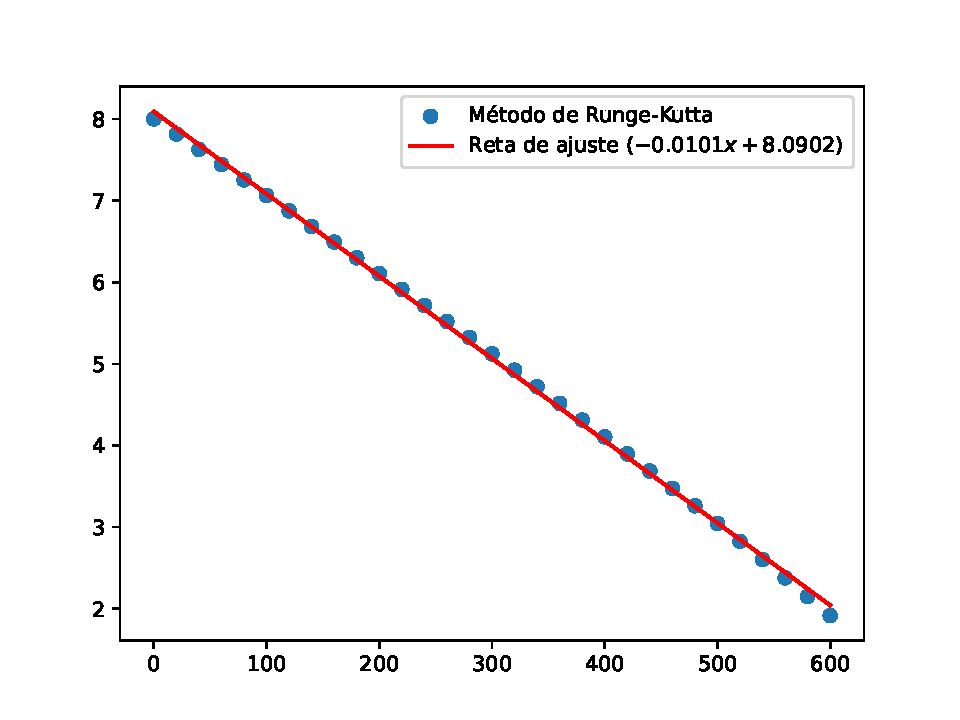
\includegraphics[width=\columnwidth]{../metodo de runge kutta/q28.pdf}
            \begin{center}
                \begin{minipage}{0.75\columnwidth}
                    Após 10 min o nível da água é de 1.9166 ft que equivale a um volume de 128.4479 $\mathrm{ft^3}$
                \end{minipage}
            \end{center}
        \end{minipage}
        \vspace{5pt}

        \item Determine, com precisão de $1 \,\mathrm{min}$ quando o tanque ficará vazio.

        Pela reta de ajuste $-0.0101x + 8.0902$, o tanque ficará vazio em $t = 802 \,\mathrm{s}$ ou aproximadamente $13 \,\mathrm{min}$.
    \end{enumerate}
\end{enumerate}
\setcounter{section}{8}
\section{EDOs de ordem superior e sistemas}
% [explicação]
\begin{enumerate}[leftmargin=*]
    \item Use o método de Runge-Kutta para sistemas para encontrar aproximações das soluções dos seguintes sistemas de equações diferenciais de primeira ordem e compare os resultados com as soluções reais
    \begin{enumerate}[leftmargin=*]
        \item[a.] 
        $
        \left\{
        \begin{array}{ll}
            u_1' = 3u_1 + 2u_2 - (2t^2 + 1)e^{2t} & u_1 (0) = 1\\
            u_2' = 4u_1 + u_2 + (t^2 + 2t - 4)e^{2t} & u_2(0) = 1
        \end{array}
        \right.
        $
        $0 \leqslant t \leqslant 1$ e $h = 0.2$
        \vspace{5pt}

        \begin{minipage}{0.45\columnwidth}
            \begin{tblr}{
                colspec={crrc},
                hline{1,Z} = {1pt, solid},
                hline{2} = {0.5pt, solid},
                row{1} = {c, abovesep=3pt, belowsep=3pt}
                }   
                $t_i$ & $w_i^1$   & $u_1(t_i)$ & $|u_1(t_i) - w_i^1|$\\
                0.0   &  1.0000  &  1.0000   & 0.0000 \\
                0.2   &  2.1204  &  2.1250   & 0.0046 \\
                0.4   &  4.4412  &  4.4651   & 0.0239 \\
                0.6   &  9.7391  &  9.8324   & 0.0932 \\
                0.8   & 22.6766  & 23.0026   & 0.3261 \\
                1.0   & 55.6612  & 56.7375   & 1.0763 \\
            \end{tblr}
        \end{minipage}
        \hfill
        \begin{minipage}{0.45\columnwidth}
            \begin{tblr}{
                colspec={crrc},
                hline{1,Z} = {1pt, solid},
                hline{2} = {0.5pt, solid},
                row{1} = {c, abovesep=3pt, belowsep=3pt}
                }   
                $t_i$ & $w_2^i$   & $u_2(t_i)$ & $|u_2(t_i) - w_2^i|$\\
                0.0   &  1.0000  &  1.0000   & 0.0000 \\
                0.2   &  1.5070  &  1.5116   & 0.0046 \\
                0.4   &  3.2422  &  3.2660   & 0.0237 \\
                0.6   &  8.1634  &  8.2563   & 0.0929 \\
                0.8   & 21.3435  & 21.6689   & 0.3253 \\
                1.0   & 56.0305  & 57.1054   & 1.0749 \\
            \end{tblr}
        \end{minipage}
        \begin{center}
            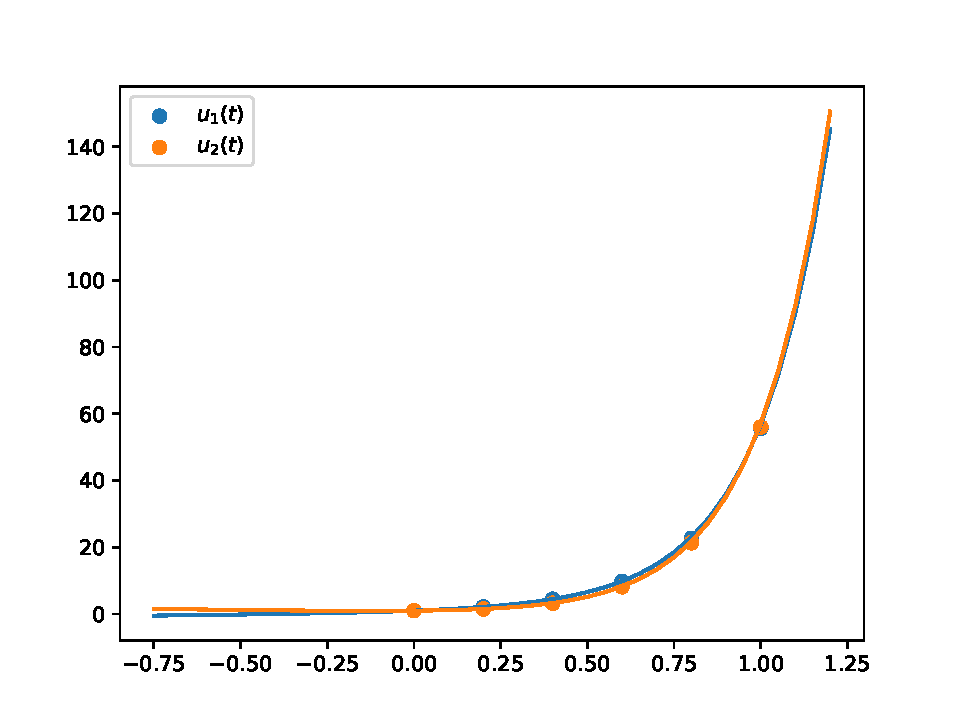
\includegraphics[width=0.65\textwidth]{../sistemas de edos/q1a.pdf}
        \end{center}

        \item[b.]
        $
        \left\{
        \begin{array}{ll}
            u_1' = -4u_1 - 2u_2 + \cos t + 4 \sin t & u_1 (0) = 0\\
            u_2' =  3u_1 + u_2 - 3 \sin t & u_2(0) = -1
        \end{array}
        \right.
        $
        $0 \leqslant t \leqslant 1$ e $h = 0.1$
        \vspace{5pt}

        \begin{minipage}{0.45\columnwidth}
            \begin{tblr}{
                colspec={crrc},
                hline{1,Z} = {1pt, solid},
                hline{2} = {0.5pt, solid},
                row{1} = {c, abovesep=3pt, belowsep=3pt}
                }   
                $t_i$ & $w_i^1$   & $u_1(t_i)$ & $|u_1(t_i) - w_i^1|$\\
                0.0 & 0.00000 & 0.00000 & 0.00000 \\
                0.1 & 0.27204 & 0.27205 & 0.00001 \\
                0.2 & 0.49548 & 0.49549 & 0.00001 \\
                0.3 & 0.67952 & 0.67953 & 0.00001 \\
                0.4 & 0.83139 & 0.83140 & 0.00001 \\
                0.5 & 0.95671 & 0.95673 & 0.00001 \\
                0.6 & 1.05986 & 1.05988 & 0.00001 \\
                0.7 & 1.14418 & 1.14419 & 0.00001 \\
                0.8 & 1.21221 & 1.21222 & 0.00002 \\
                0.9 & 1.26585 & 1.26587 & 0.00001 \\
                1.0 & 1.30654 & 1.30656 & 0.00001 \\
                1.1 & 1.33533 & 1.33534 & 0.00001 \\
                1.2 & 1.35298 & 1.35299 & 0.00001 \\
                1.3 & 1.36006 & 1.36007 & 0.00001 \\
                1.4 & 1.35701 & 1.35702 & 0.00001 \\
                1.5 & 1.34417 & 1.34418 & 0.00001 \\
                1.6 & 1.32183 & 1.32184 & 0.00001 \\
                1.7 & 1.29027 & 1.29029 & 0.00001 \\
                1.8 & 1.24978 & 1.24980 & 0.00001 \\
                1.9 & 1.20068 & 1.20070 & 0.00001 \\
                2.0 & 1.14332 & 1.14334 & 0.00001 \\
            \end{tblr}
        \end{minipage}
        \hfill
        \begin{minipage}{0.45\columnwidth}
            \begin{tblr}{
                colspec={crrc},
                hline{1,Z} = {1pt, solid},
                hline{2} = {0.5pt, solid},
                row{1} = {c, abovesep=3pt, belowsep=3pt}
                }   
                $t_i$ & $w_2^i$   & $u_2(t_i)$ & $|u_2(t_i) - w_2^i|$\\
                0.0 & -1.00000 & -1.00000 & 0.00000\\
                0.1 & -1.07705 & -1.07705 & 0.00001\\
                0.2 & -1.11554 & -1.11555 & 0.00001\\
                0.3 & -1.12482 & -1.12483 & 0.00001\\
                0.4 & -1.11229 & -1.11230 & 0.00001\\
                0.5 & -1.08382 & -1.08383 & 0.00001\\
                0.6 & -1.04403 & -1.04405 & 0.00001\\
                0.7 & -0.99655 & -0.99656 & 0.00001\\
                0.8 & -0.94418 & -0.94419 & 0.00001\\
                0.9 & -0.88910 & -0.88911 & 0.00001\\
                1.0 & -0.83295 & -0.83297 & 0.00001\\
                1.1 & -0.77699 & -0.77701 & 0.00001\\
                1.2 & -0.72213 & -0.72215 & 0.00001\\
                1.3 & -0.66903 & -0.66905 & 0.00001\\
                1.4 & -0.61816 & -0.61817 & 0.00001\\
                1.5 & -0.56980 & -0.56982 & 0.00001\\
                1.6 & -0.52415 & -0.52417 & 0.00001\\
                1.7 & -0.48129 & -0.48130 & 0.00001\\
                1.8 & -0.44124 & -0.44125 & 0.00001\\
                1.9 & -0.40395 & -0.40396 & 0.00001\\
                2.0 & -0.36936 & -0.36937 & 0.00001\\
            \end{tblr}
        \end{minipage}
        \begin{center}
            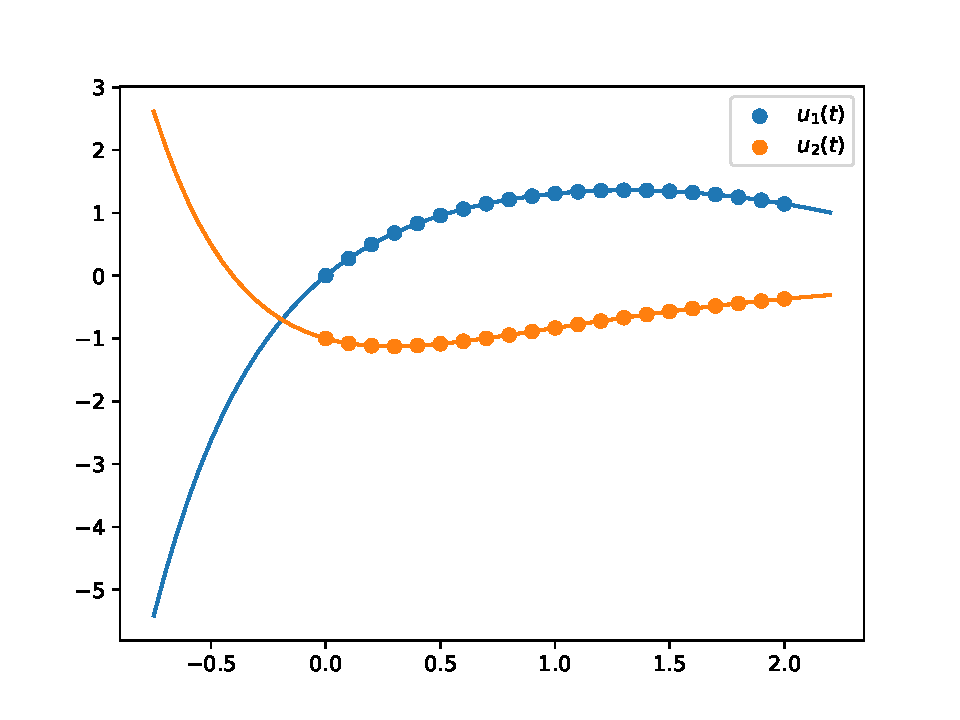
\includegraphics[width=0.65\textwidth]{../sistemas de edos/q1b.pdf}
        \end{center}

        \item[d.] 
        $
        \left\{
        \begin{array}{ll}
            u_1' = u_2 - u_3 + t & u_1 (0) = 1\\
            u_2' =  3t^2 & u_2(0) = 1\\
            u_3' = u_2 + e^{-t}  & u_2(0) = -1\\
        \end{array}
        \right.
        $
        $0 \leqslant t \leqslant 1$ e $h = 0.1$
        \vspace{5pt}

        \begin{minipage}{0.45\columnwidth}
            \begin{tblr}{
                width=\columnwidth,
                colspec={crrc},
                hline{1,Z} = {1pt, solid},
                hline{2} = {0.5pt, solid},
                row{1} = {c, abovesep=3pt, belowsep=3pt}
                }   
                $t_i$ & $w_1^i$   & $u_1(t_i)$ & $|u_1(t_i) - w_1^i|$\\
                0.0 & 1.00000 & 1.00000 & 0.00000 \\
                0.1 & 1.00100 & 1.00100 & 0.00000 \\
                0.2 & 1.00800 & 1.00800 & 0.00000 \\
                0.3 & 1.02700 & 1.02700 & 0.00000 \\
                0.4 & 1.06400 & 1.06400 & 0.00000 \\
                0.5 & 1.12500 & 1.12500 & 0.00000 \\
                0.6 & 1.21600 & 1.21600 & 0.00000 \\
                0.7 & 1.34300 & 1.34300 & 0.00000 \\
                0.8 & 1.51200 & 1.51200 & 0.00000 \\
                0.9 & 1.72900 & 1.72900 & 0.00000 \\
                1.0 & 2.00000 & 2.00000 & 0.00000 \\
            \end{tblr}
        \end{minipage}
        \hfill
        \begin{minipage}{0.45\columnwidth}
            \begin{tblr}{
                width=\columnwidth,
                colspec={crrc},
                hline{1,Z} = {1pt, solid},
                hline{2} = {0.5pt, solid},
                row{1} = {c, abovesep=3pt, belowsep=3pt}
                }   
                $t_i$ & $w_2^i$   & $u_2(t_i)$ & $|u_2(t_i) - w_2^i|$\\
                0.0 & 1.00000 & 1.00000 & 0.00000 \\
                0.1 & 1.19519 & 1.19519 & 0.00000 \\
                0.2 & 1.38165 & 1.38165 & 0.00000 \\
                0.3 & 1.56108 & 1.56109 & 0.00000 \\
                0.4 & 1.73557 & 1.73557 & 0.00000 \\
                0.5 & 1.90753 & 1.90753 & 0.00000 \\
                0.6 & 2.07970 & 2.07970 & 0.00000 \\
                0.7 & 2.25504 & 2.25504 & 0.00000 \\
                0.8 & 2.43669 & 2.43669 & 0.00000 \\
                0.9 & 2.62793 & 2.62793 & 0.00000 \\
                1.0 & 2.83212 & 2.83212 & 0.00000 \\
            \end{tblr}
        \end{minipage}
        \begin{center}
            \begin{tblr}{
                colspec={crrc},
                width=\columnwidth,
                hline{1,Z} = {1pt, solid},
                hline{2} = {0.5pt, solid},
                row{1} = {c, abovesep=3pt, belowsep=3pt}
                }   
                $t_i$ & $w_3^i$   & $u_3(t_i)$ & $|u_3(t_i) - w_3^i|$\\
                0.0 & -1.00000 & -1.00000 & 0.00000 \\
                0.1 & -0.80481 & -0.80481 & 0.00000 \\
                0.2 & -0.61833 & -0.61833 & 0.00000 \\
                0.3 & -0.43879 & -0.43879 & 0.00000 \\
                0.4 & -0.26392 & -0.26392 & 0.00000 \\
                0.5 & -0.09091 & -0.09091 & 0.00000 \\
                0.6 & 0.08359 & 0.08359 & 0.00000 \\
                0.7 & 0.26344 & 0.26344 & 0.00000 \\
                0.8 & 0.45307 & 0.45307 & 0.00000 \\
                0.9 & 0.65746 & 0.65746 & 0.00000 \\
                1.0 & 0.88212 & 0.88212 & 0.00000 \\
            \end{tblr}
        \end{center}
        \begin{center}
            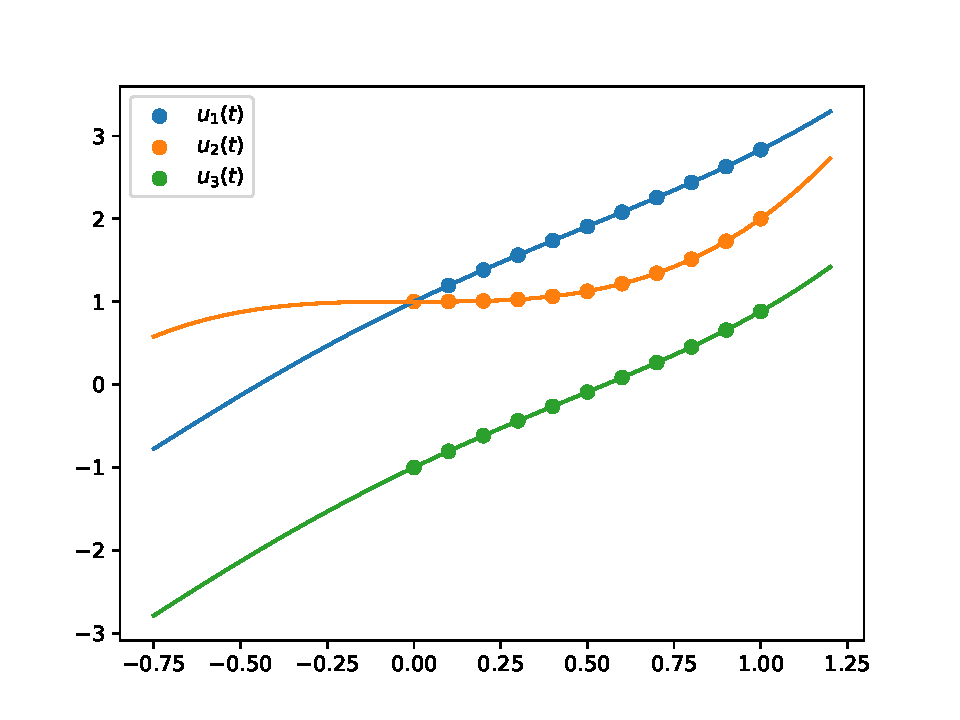
\includegraphics[width=0.7\textwidth]{../sistemas de edos/q1d.pdf}
        \end{center}
    \end{enumerate}

    \item[3.] Use o algoritmo de Runge-Kutta para sistemas para encontrar aproximações das seguintes equações diferenciais e compare com os resultados das soluções reais
    \begin{enumerate}[leftmargin=*]
        \item $y'' - 2y' + y = te^t - t$, $\;0 \leqslant t \leqslant 1$, $\; y(0) = y'(0) = 0$ com $h = 0.1$ \\[3.5pt] solução exata: $y(t) = \frac{1}{6}t^3 e^t - te^t + 2e^t -2$.

        Transformando em um sistema, temos
        \[
            \left\{
            \begin{array}{ll}
                x' = 2x - y - te^t - t & x(0) = 0\\
                y' = x & y(0) = 0\\
            \end{array}
            \right.
        \]
        \begin{minipage}{0.42\columnwidth}
            \begin{tblr}{
                colspec={crrc},
                hline{1,Z} = {1pt, solid},
                hline{2} = {0.5pt, solid},
                row{1} = {c, abovesep=3pt, belowsep=3pt}
                }   
                $t_i$ & $w_i$   & $y(t_i)$ & $|y(t_i) - w_i|$\\
                0.0 & 0.00000 & 0.00000 & 0.00000\\
                0.1 & 0.00001 & 0.00001 & 0.00000\\
                0.2 & 0.00015 & 0.00015 & 0.00000\\
                0.3 & 0.00083 & 0.00083 & 0.00000\\
                0.4 & 0.00283 & 0.00283 & 0.00000\\
                0.5 & 0.00743 & 0.00743 & 0.00000\\
                0.6 & 0.01656 & 0.01656 & 0.00000\\
                0.7 & 0.03300 & 0.03300 & 0.00000\\
                0.8 & 0.06056 & 0.06056 & 0.00000\\
                0.9 & 0.10440 & 0.10441 & 0.00000\\
                1.0 & 0.17132 & 0.17133 & 0.00001\\
            \end{tblr}
        \end{minipage}
        \hfill
        \begin{minipage}{0.53\columnwidth}
            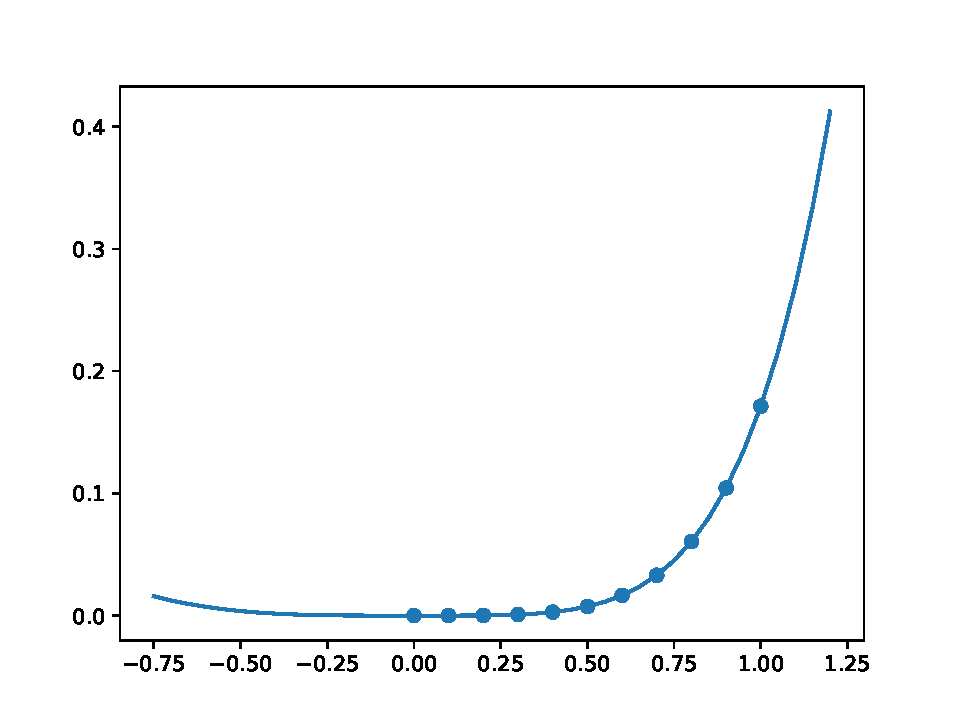
\includegraphics[width=\columnwidth]{../sistemas de edos/q3a.pdf}
        \end{minipage}
    \end{enumerate}
\end{enumerate}

\setcounter{chapter}{1}
\setcounter{section}{0}
\renewcommand\thechapter{\Alph{chapter}}
\section{Algoritmos para EDOs}
\begin{minted}[autogobble, mathescape]{python}
        def part(N, tmin, tmax):
            h = (tmax - tmin)/N
            
            t = np.zeros(N+1)
            for i in range(len(t)):
                t[i] = tmin + i*h
            
            return t
\end{minted}
\begin{minted}[autogobble, mathescape]{python}
        def metodo_de_euler(g, N, y, tmin, tmax):
            def f(t,x):
                f = eval(gx)
                return f
    
            h = (tmax - tmin)/N
            t = part(N, tmin, tmax)
            w = np.zeros(N+1)
            
            w[0] = y
            for i in range(1,len(w)):
                w[i] = w[i-1] + h*f(t[i-1], w[i-1]) # $w_i = w_{i-1} + hf(t_{i-1}, w_{i-1})$
                
            return w,t
\end{minted}
\begin{minted}[autogobble, mathescape]{python}
    def metodo_de_taylor_ordem_2(N,y, tmin, tmax):
        h = (tmax - tmin)/N
        
        t = part(N, tmin, tmax)
        
        w = np.zeros(N+1)
        
        w[0] = y
        for i in range(1,len(w)):
            w[i] = w[i-1] + h*(f(t[i-1], w[i-1])) + 0.5*(h**2)*df(t[i-1], w[i-1])
            
        return w,t
\end{minted}
\begin{minted}[autogobble, mathescape]{python}
    def metodo_de_runge_kutta(N, y, tmin, tmax):
        h = (tmax - tmin)/N
        t = part(N, tmin, tmax)
        w = np.zeros(N+1)
        
        w[0] = y
        
        for i in range(1, len(w)):
            K1 = h*f(t[i-1], w[i-1])
            K2 = h*f(t[i-1] + 0.5*h, w[i-1] + 0.5*K1)
            K3 = h*f(t[i-1] + 0.5*h, w[i-1] + 0.5*K2)
            K4 = h*f(t[i], w[i-1] + K3)
            
            w[i] = w[i-1] + (K1 + 2*K2 + 2*K3 + K4)*(1/6)
            
        return w, t
\end{minted}
\begin{minted}[autogobble, mathescape]{python}
    def metodo_de_euler_modificado(N,y, tmin, tmax):
        w[0] = y
        for i in range(1,len(w)):
            w[i] = w[i-1] + 0.5*h*(f(t[i-1],w[i-1]) + f(t[i], w[i-1] + h*f(t[i-1], w[i-1])))
            
        return w,t    
\end{minted}
\begin{minted}[autogobble, mathescape]{python}
    def metodo_do_ponto_medio(N,y, tmin, tmax):
        w[0] = y
        for i in range(1,len(w)):
            w[i] = w[i-1] + h*f(t[i-1] + 0.5*h, w[i-1] + 0.5*h*f(t[i-1],w[i-1]))
            
        return w,t    
\end{minted}
\begin{minted}[autogobble, mathescape]{python}
    def metodo_de_runge_kutta(N, y, tmin, tmax): # para sistemas de duas EDOs
        h = (tmax - tmin)/N
        t = part(N, tmin, tmax)
        w = np.zeros((N+1,2))
        
        w[0,:] = y
        
        for i in range(1, len(w)):
            K1 = h*f(t[i-1], w[i-1,0], w[i-1,1])
            K2 = h*f(t[i-1] + 0.5*h, w[i-1,0] + 0.5*K1[0], w[i-1,1] + 0.5*K1[1])
            K3 = h*f(t[i-1] + 0.5*h, w[i-1,0] + 0.5*K2[0], w[i-1,1] + 0.5*K2[1])
            K4 = h*f(t[i], w[i-1,0] + K3[0], w[i-1,1] + K3[1])
            
            w[i] = w[i-1] + (K1 + 2*K2 + 2*K3 + K4)*(1/6)
            
        return w, t
\end{minted}
\section{Algoritmos para interpolação}
\begin{minted}[autogobble]{python}
    def neville(A,x):
        X = A[:,0]
        Y = A[:,1]
        
        n = len(A)
        
        B = np.zeros((n,n))
        
        B[:,0] = Y
        
        for i in range(1,n):
            for j in range(1, i + 1):
                B[i,j] = (((x - X[i-j])*B[i,j-1])
                - ((x - X[i])*B[i-1,j-1]))/(X[i]-X[i-j])
        
        for i in range(n):
            for j in range(n):
                print(f'{B[i,j]:.3f}', end='\t')
            print("")
            
        print(f"Solução aproximada para {x} ::: {B[n-1,n-1]}")
\end{minted}

\end{document}